
\documentclass{report}

\usepackage[french]{babel}
\usepackage[T1]{fontenc}
\usepackage[letterpaper,top=2cm,bottom=2cm,left=3cm,right=3cm,marginparwidth=1.75cm]{geometry}
\usepackage{amsmath}
\usepackage{graphicx}
\usepackage{enumitem}
\usepackage{subfig}
\usepackage{float}
\usepackage{array}
\usepackage{longtable}

\usepackage[colorlinks=true, allcolors=blue]{hyperref}

\title{Tetris Royale : SRD \\ INFO-F—209 : Projet d'Informatique 2}

\author{
Ali Umar Babar \and
Ayman Benaim \and
Antoine Berthion \and
Mamadou Barry \and
Oleksandra Omelyanyuk \and
Rares Bors \and
Roberto Rabei \and
Taha Es-saâdouni
}

\begin{document}
\maketitle
\tableofcontents

\chapter{Introduction}
\label{chap:intro}
\section{Objectif du SRD}

Ce document de spécifications des besoins logiciels (\textit{Software Requirements Document}, \textbf{SRD}) vise à décrire les exigences et les aspects clés du projet "Tetris Royale", réalisé dans le cadre du cours d'informatique \textit{INFO-F209}. \\

\noindent L'objectif principal de ce rapport est de fournir une vision claire et structurée des besoins logiciels, des choix architecturaux, et des outils utilisés pour le développement. Par ailleurs, des diagrammes explicatifs suivant les conventions \textbf{UML} (\textit{Unified Modeling Language}) seront présentés afin d'illustrer l'implémentation technique et les interactions entre les différentes composantes du projet. \\

\noindent Cette introduction constitue une vue d'ensemble des thèmes abordés dans le document, servant ainsi de guide pour comprendre la portée et les objectifs du projet.

\section{Description du Projet}
\label{sec:description}

\subsection{Résumé}
\noindent Le projet consiste à développer \textbf{Tetris Royale}, une version multijoueur compétitive du jeu classique \emph{Tetris}. Chaque joueur place des pièces (\emph{tetraminos}) tombant sur une grille en essayant de compléter des lignes horizontales. Lorsqu'une ligne est complétée, elle disparaît et le joueur gagne des points. \emph{Tetris Royale} se distingue des autres versions de \emph{Tetris} en permettant aux joueurs d'envoyer des malus à leurs adversaires sous forme de lignes incomplètes supplémentaires lorsqu'ils complètent plusieurs lignes en un seul coup. Le but du jeu est de survivre le plus longtemps possible. Le dernier joueur en lice, après élimination de tous les autres, est déclaré vainqueur.

\subsection{Modes de jeu}
\noindent Quatre modes de jeu sont disponibles : \emph{Endless}, \emph{Classic}, \emph{Duel} et \emph{Royal Competition}.

\subsubsection{Mode Endless}
\noindent Le mode \emph{Endless} est un mode à joueur unique. Le joueur gagne des points en fonction de ses combos, tandis que la vitesse de chute des pièces augmente progressivement. Le score final est enregistré dans un classement en ligne.

\subsubsection{Mode Classic}
\noindent Le mode \emph{Classic} permet à un groupe de 3 à 9 joueurs de s’affronter dans des parties simples, où seuls des malus basiques sont utilisés (ces derniers seront décrits dans une section ultérieure). Le dernier joueur en lice est déclaré gagnant.

\subsubsection{Mode Duel}
\noindent Le mode \emph{Duel} suit les mêmes règles que le mode \emph{Classic}, mais se joue en un contre un.

\subsubsection{Mode Royal Competition}
\noindent Dans le mode \emph{Royal Competition}, les malus ne sont plus envoyés automatiquement. Les joueurs accumulent de l'énergie, et lorsqu’ils en ont suffisamment, ils peuvent choisir d'envoyer un malus ou de s’octroyer un bonus (ces mécanismes seront détaillés ultérieurement). Ce mode se joue, comme le mode \emph{Classic}, en groupes de 3 à 9 joueurs.

\subsection{Fonctionnalités multijoueurs}
\noindent Dans les modes multijoueurs, chaque joueur peut visualiser les tableaux des autres participants.

\subsection{Fonctionnalités hors partie}
\noindent En dehors des parties, le joueur dispose des fonctionnalités suivantes :
\begin{itemize}
    \item Gérer son compte ;
    \item Consulter une liste d'amis pour discuter ou inviter des joueurs en tant que participants ou observateurs ;
    \item Créer ou rejoindre une partie ;
    \item Consulter le classement des meilleurs joueurs du mode \emph{Endless}.
\end{itemize}

\section{Glossaire}

\noindent Dans cette courte section, nous définirons quelques mots que nous utiliserons au long de ce \textbf{SRD}. Ce glossaire est composé d'éléments liés à \textit{Tetris Royale}, et plus généralement au développement de celui-ci.

\begin{itemize}
    \item\textbf{Pseudo} : Nom d’utilisateur choisi par celui-ci lors de la création de son compte.
    \item\textbf{Combo} : Action de compléter plusieurs lignes simultanément.
    \item\textbf{Matchmaking} : Mécanisme de mise en relation des joueurs afin de créer une partie en ligne.
    \item\textbf{Lobby} : Interface ou lieu où l'on regroupe des joueurs avant de démarrer une partie.
    \item\textbf{User (Utilisateur)} : Client qui est connecté en réseau et lié à un compte.
    \item\textbf{Tetramino} : Pièce de \emph{Tetris}, composée de 4 blocs carrés disposés selon diverses configurations.
    \item\textbf{Battle Royale} : Mode de compétition où chaque joueur s'affronte pour être le dernier en vie.
    \item\textbf{Ligne} : Une rangée complète de blocs horizontaux sur la grille. Une ligne complétée disparaît.
    \item\textbf{Grille} : L'aire de jeu où tombent les \emph{tetraminos}. Elle mesure 10 cases de large et 22 cases de haut.
    \item\textbf{Tetris} : Compléter quatre lignes en une seule action à l’aide d’une pièce en forme de barre (\emph{I}).
\end{itemize}



\section{Historique}

\noindent Dans cette courte section, nous présenterons un historique des différentes versions ce ce \textbf{SRD}. La figure ci-dessous illustre l'évolution du document.

\begin{longtable}{
|>{\centering\arraybackslash}m{2cm}|>{\centering\arraybackslash}m{4cm}|m{7cm}|>{\centering\arraybackslash}m{3cm}|}
\hline
\textbf{Version} & \textbf{Nom} & \textbf{Modifications} & \textbf{Date} \\ \hline
\endfirsthead
\hline
\textbf{Version} & \textbf{Nom} & \textbf{Modifications} & \textbf{Date} \\ \hline
\endhead
0.1 & Oleksandra Omelyanyuk & Introduction + besoins utilisateurs & 05/12/2024 \\ \hline
0.2 & Roberto Rabei & Besoins système & 08/12/2024 \\ \hline
0.3 & Roberto Rabei & Squelette Design système & 09/12/2024 \\ \hline
0.4 & Oleksandra Omelyanyuk & Modifications besoins système + diagrammes & 09/12/2024 \\ \hline
1.0 & Berthion Antoine & Restructuration du SRD & 13/12/2024 \\ \hline
1.1 & Oleksandra Omelyanyuk & Début adaptation aux changements & 10/03/2025 \\ \hline
1.2 & Oleksandra Omelyanyuk & Modification/rajout diagrammes & 12/03/2025 \\ \hline
\end{longtable}



\chapter{Besoins Utilistateurs}
\label{chap:user_req}

Dans cette section du SRD, il s'agira de décrire les besoins spécifiques à l'utilisateur. En particulier, nous distinguerons les besoins fonctionnels, c'est-à-dire les exigences techniques et liées à l'implémentation du \emph{Tetris Royale}, ainsi que les besoins non-fonctionnels, qui concernent l'expérience utilisateur et les attentes en termes de performance, de sécurité et d'ergonomie.

\section{Besoins Fonctionnels}
\subsection{Connexion et Création de Compte}

\noindent Lorsque l’utilisateur lance le jeu, il est d'abord accueilli par une fenêtre de connexion. Cette fenêtre lui permet de se connecter à son compte en saisissant son identifiant et son mot de passe. Si l'utilisateur ne possède pas encore de compte, il a la possibilité d'en créer un en cliquant sur un bouton de création de compte. \\

\noindent Lors de la création d'un compte, l'utilisateur doit fournir les informations suivantes :
\begin{itemize}
    \item \textbf{Pseudo} : L'utilisateur doit choisir un pseudo qui lui est unique. Le système vérifiera que le pseudo choisi n'est pas déjà utilisé par un autre joueur.
    \item \textbf{Mot de Passe} : L'utilisateur doit également choisir un mot de passe sécurisé pour protéger son compte. Le mot de passe sera requis pour la connexion ultérieure.
    \item \textbf{Validation du Pseudo} : Si le pseudo choisi est déjà pris, l'utilisateur recevra un message d'erreur lui demandant de choisir un autre pseudo. Une fois un pseudo disponible sélectionné, l'utilisateur pourra poursuivre la création de son compte. \\
\end{itemize}

\vspace{-2em}

\begin{figure}[H]
    \centering
     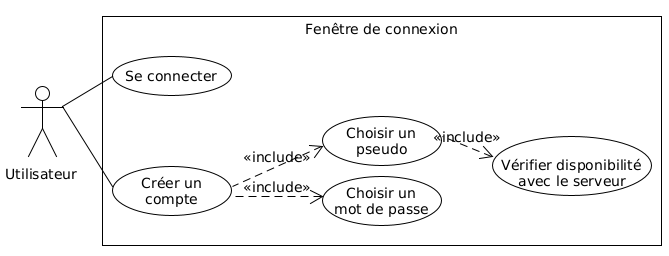
\includegraphics[width=0.5\textwidth, keepaspectratio]{src/user_req/connexion.png}
    \caption{Use-Case : Connexion et Création de Compte}
    \label{fig:use_case_connexion}
\end{figure}

\noindent Une fois ces informations validées, le compte est créé et l'utilisateur est connecté à son profil. Le joueur peut alors accéder aux différentes fonctionnalités du jeu, telles que rejoindre des parties, consulter ses statistiques et interagir avec d'autres utilisateurs.

\noindent Si l'utilisateur a déjà un compte, il peut simplement saisir ses identifiants (pseudo et mot de passe) pour se connecter.



\subsection{Gestion des Parties et Profil Utilisateur}

\noindent Cette sous-section décrit en détail les interactions disponibles pour l'utilisateur via l'interface du menu, illustrée dans la figure \ref{fig:use_case_menu} ci-dessous. 

\vspace{-1em}

\begin{figure}[H]
    \centering
     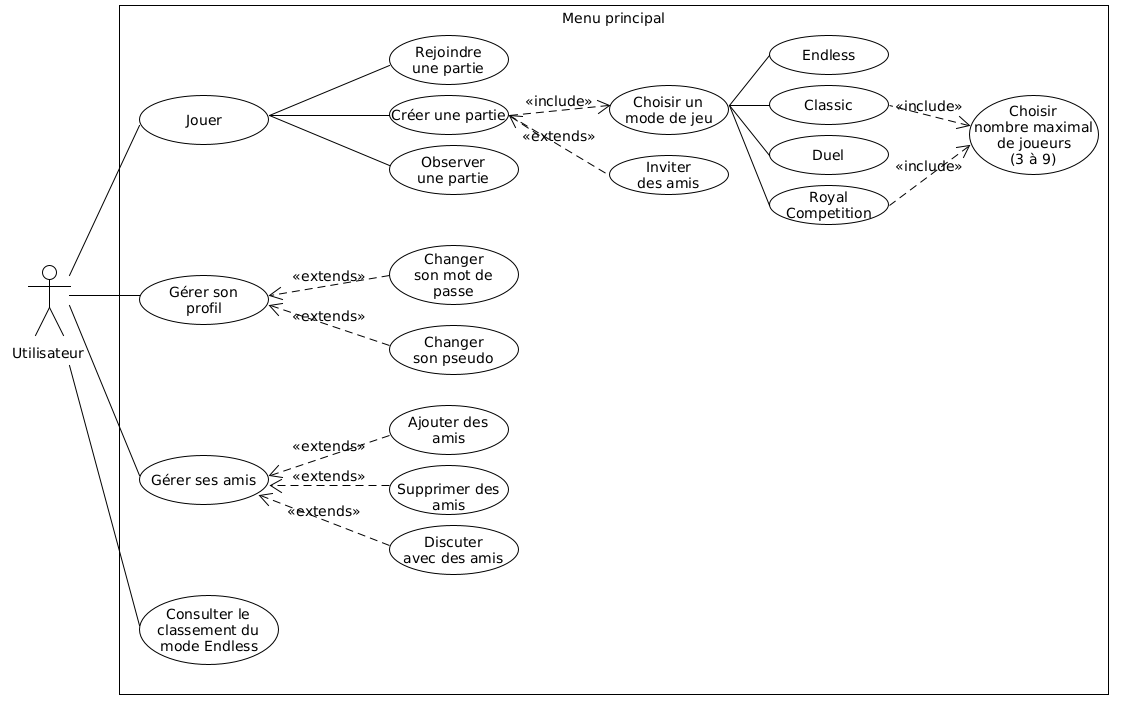
\includegraphics[width=0.9\textwidth, keepaspectratio]{src/user_req/menu.png}
    \caption{Use-Case : Menu Principal}
    \label{fig:use_case_menu}
\end{figure}

\noindent Lorsque l'utilisateur décide de jouer, il peut choisir entre rejoindre une partie déjà créée ou créer sa propre partie.

\subsubsection{Création de Partie}

\noindent Si l'utilisateur choisit de créer sa propre partie, il dispose des options suivantes :
\begin{itemize}
    \item \textbf{Inviter des amis} : L'utilisateur peut inviter ses amis à participer à la partie, soit pour jouer, soit pour observer. Une invitation correspond à un code que le joueur invité devra rentrer pour accéder au jeu.
    \item \textbf{Choisir un mode de jeu} : L'utilisateur doit obligatoirement sélectionner un mode de jeu avant de lancer la partie. Il doit ensuite se mettre prêt, en attendant que le bon nombre de joueurs rejoigne sa partie.
    \item \textbf{Choisir un nombre maximal de joueurs} : Pour les modes \emph{Classic} et \emph{Royal Competition}, l'utilisateur doit définir un nombre maximal de joueurs qui peuvent rejoindre la partie. Ce nombre doit être compris entre 3 et 9 joueurs inclus.
\end{itemize}

\subsubsection{Rejoindre une Partie}

\noindent L'utilisateur peut également choisir de rejoindre une partie existante. Il peut accéder à un menu contenant les parties en cours, ou qui n'ont pas encore atteint leur nombre souhaité de joueurs, et peut alors choisir de les rejoindre ou de les observer.

\subsubsection{Gestion du Profil Utilisateur}

\noindent Chaque utilisateur possède un profil qui lui est associé. Il peut y accéder à tout moment pour effectuer certaines actions de gestion personnelle :
\begin{itemize}
    \item \textbf{Modifier son mot de passe} : L'utilisateur peut changer son mot de passe à tout moment pour renforcer la sécurité de son compte.
    \item \textbf{Modifier son pseudo} : L'utilisateur peut également changer son pseudo. Cependant, le nouveau pseudo sera accepté uniquement s'il est disponible, c'est-à-dire s'il n'est pas déjà pris par un autre joueur.
\end{itemize}

\subsubsection{Liste d'Amis et Discussions}

\noindent Chaque utilisateur possède une liste d'amis, qu'il peut gérer de la manière suivante :

\begin{itemize}
    \item \textbf{Ajouter des amis} : L'utilisateur peut envoyer des demandes d'ami à d'autres joueurs. Une fois la demande acceptée, ils deviennent amis et peuvent interagir dans le jeu.
    \item \textbf{Supprimer des amis} : L'utilisateur peut retirer des amis de sa liste à tout moment.
    \item \textbf{Lancer une discussion} : L'utilisateur peut démarrer une conversation avec un ami à partir de la liste d'amis.
\end{itemize}

\subsubsection{Classement du Mode Endless}

\noindent L'utilisateur peut accéder à un classement en ligne des joueurs du mode \emph{Endless}. Ce classement présente tous les joueurs ainsi que leurs scores, classés dans l'ordre décroissant. Cela permet à l'utilisateur de voir sa position par rapport aux autres joueurs et de suivre la progression des meilleurs joueurs du mode.





\subsection{Déroulement d’une partie}

\noindent Une fois que le joueur a lancé une partie, il peut déplacer un tetramino pour le positionner sur son tableau de jeu. Il peut également utiliser le \emph{bag}, un espace dans lequel il peut ranger un tetramino ou utiliser celui qui y est déjà stocké. \\

\noindent De plus, le joueur a la possibilité d'utiliser des malus, mais seulement s'il joue dans les modes \emph{Classic}, \emph{Duel} ou \emph{Royal Competition} (dans ce mode des bonus sont aussi disponibles). Dans ces trois modes, il peut également voir les tableaux des autres joueurs en temps réel.

\begin{figure}[H]
    \centering
     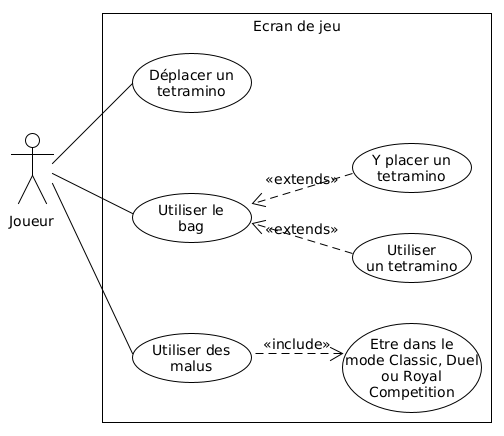
\includegraphics[width=0.4\textwidth, keepaspectratio]{src/user_req/jeu.png}
    \caption{Use-Case : Déroulement d'une partie}
    \label{fig:use_case_game}
\end{figure}

\subsubsection{Malus et bonus}

\noindent Dans les modes de jeu autres que \emph{Royal Competition}, où des bonus et des malus avancés sont disponibles, seuls des malus basiques sont envoyés automatiquement lorsqu'un joueur réalise un combo. Ces malus se traduisent par l'apparition de lignes additionnelles sur le tableau d'un joueur adverse, selon les règles suivantes :
\begin{itemize}
    \item 1 ligne complétée n'envoie aucun malus.
    \item 2 lignes complétées envoient 1 ligne de malus.
    \item 3 lignes complétées envoient 2 lignes de malus.
    \item 4 lignes complétées (Tetris) envoient 4 lignes de malus. \\
\end{itemize}

\vspace{-1em}

\noindent Dans le mode \emph{Classic}, le joueur peut également changer le joueur actuellement ciblé par ses malus, lui offrant ainsi un certain contrôle stratégique sur l’adversaire. \\

\vspace{-1em}

\noindent Le mode \emph{Royal Competition} introduit des malus plus avancés, incluant des bonus (avantages), permettant une interaction plus dynamique avec les autres joueurs. Voici quelques exemples des \textit{power-ups} disponibles dans ce mode :
\begin{itemize}
    \item \textbf{Inverser les commandes} : Inverse les commandes du joueur ciblé pour la pose des trois prochains blocs.
    \item \textbf{Bloquer les commandes} : Bloque les commandes du joueur ciblé pour la pose du prochain bloc.
    \item \textbf{Réduire la vitesse de chute} : Réduit la vitesse de chute des pièces sur son propre plateau pendant un moment.
    \item \textbf{Augmenter la difficulté} : Accélère la chute des pièces sur le plateau de l’adversaire.
    \item \textbf{Éclair} : Envoie un éclair qui supprime les blocs dans une zone de 2x2 chez le joueur ciblé.
    \item \textbf{Éteindre la lumière} : Éteint la lumière, rendant le tableau du joueur ciblé invisible pendant un court moment.
    \item \textbf{Blocs de 1x1} : Les deux prochaines pièces du joueur se transforment en blocs de 1x1.
\end{itemize}





\section{Besoins non-fonctionnels}

\noindent Le jeu doit offrir une interface à la fois simple d’utilisation et agréable à l’œil. Cela est particulièrement important dans les modes multijoueurs, où les tableaux des adversaires doivent être affichés de manière claire et disposés de façon à ne pas encombrer l’interface principale du jeu. C'est pourquoi il est possible d'afficher un seul tableau adverse à la fois, avec une possibilité de changer d'adversaire visé.\\ 

\noindent De plus, le jeu doit être accessible à travers différentes interfaces, permettant à l’utilisateur de jouer aussi bien sur un terminal que sur une interface graphique (GUI). \\

\noindent Un autre besoin crucial est la rapidité de l’envoi d’information entre les joueurs. Pour garantir une expérience de jeu fluide et réactive, il est essentiel qu’il n’y ait aucun délai perceptible lorsque le joueur consulte les grilles de ses adversaires.



\chapter{Besoins Systèmes}
\label{chap:sys_req}

\section{Connexion}

\noindent Le système doit permettre la création de nouveaux comptes tout en vérifiant les informations fournies par les utilisateurs. Lors de l'inscription, il doit s'assurer que le pseudonyme choisi n'est pas déjà utilisé par un autre utilisateur. Une fois les informations validées, elles doivent être enregistrées sur le serveur. Pour la connexion, le système doit vérifier l'authenticité des données en les comparant à celles stockées sur le serveur.

\vspace{-1em}

\begin{figure}[H]
    \centering
     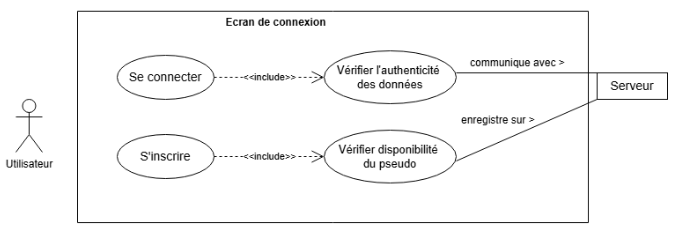
\includegraphics[width=0.9\textwidth, keepaspectratio]{src/sys_req/connexion.png}
    \caption{Use-Case : Connexion}
    \label{fig:use_case_connexion_sys_req}
\end{figure}

\section{Lobby}

\noindent Lorsqu'un joueur souhaite lancer une partie, il est d'abord placé dans un lobby. Dans cet espace, il peut inviter des amis à rejoindre sa partie. Le lobby est également accessible aux joueurs aléatoires à la recherche d'une partie. Le serveur s'assure que le nombre de joueurs minimum et maximum est respecté. Lorsque tous les joueurs sont prêts, le serveur lance la partie.

\vspace{-1em}

\begin{figure}[H]
    \centering
     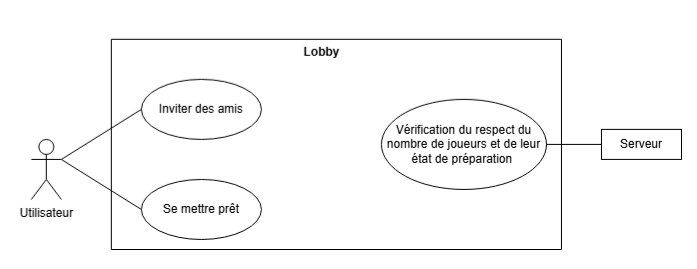
\includegraphics[width=0.8\textwidth, keepaspectratio]{src/sys_req/lobby.png}
    \caption{Use-Case : Lobby}
    \label{fig:use_case_lobby_sys_req}
\end{figure}

\section{Partie}

\noindent Le système doit être capable de suivre en temps réel les actions de chaque joueur dans la partie afin d'assurer une expérience fluide, immersive et compétitive. Selon le mode de jeu sélectionné, l'interface doit s'adapter pour offrir un affichage personnalisé :

\begin{itemize}
    \item \textbf{Endless :} Ce mode solo affiche la grille de jeu avec le nombre de points accumulés durant la partie.
    \item \textbf{Classique :} L'affichage est similaire au mode \emph{Endless}, avec, en plus, une grille d'un joueur adverse visible à droite, permettant ainsi de choisir à qui envoyer les malus.
    \item \textbf{Duel :} Le même affichage que le mode \emph{Classique}, mais sans possibilité de changer d'adversaire visé (car il y en a qu'un).
    \item \textbf{Royal Competition :} L'affichage du mode \emph{Classique} est utilisé, mais cette fois, l'utilisateur peut choisir d'utiliser des bonus ou d'envoyer des malus plus avancés, sans pouvoir envoyer le malus de base.
\end{itemize}




\chapter{Design et Fonctionnement}
\label{chap:design}

\section*{Design du système}

\noindent Le système est divisé en sept entités principales, chacune ayant un rôle précis dans le fonctionnement global du jeu. Ces entités sont :  
\begin{itemize}
    \item Connexion et Inscription
    \item Gestion des comptes
    \item Profil
    \item Menu principal
    \item Matchmaking
    \item Chat
    \item Jeu
\end{itemize}

\noindent Ces entités partagent une structure commune, en raison de l'utilisation du design \emph{MVC} (Modèle-Vue-Contrôleur). Chaque entité du système est composée de trois composants principaux :  
\begin{itemize}
    \item \textbf{La vue :} Elle correspond à l'interface utilisateur. Elle permet d'afficher les informations à l'utilisateur et de recevoir ses inputs qu'elle transmet au contrôleur.  
    \item \textbf{Le contrôleur :} Il gère les requêtes envoyées par la vue et les communique au serveur. Il met à jour le serveur en fonction des actions des utilisateurs.  
    \item \textbf{Le serveur :} Il contient toutes les informations relatives aux utilisateurs et aux parties en cours. Il est responsable d'envoyer les informations requises par le contrôleur et de mettre les joueurs en relation pour la création de parties.
\end{itemize}

\section{Connexion et inscription}

\noindent Lorsqu'un joueur démarre le jeu, il peut choisir entre créer un nouveau compte ou se connecter à un compte existant. Deux interfaces distinctes sont proposées pour ces actions. Lors de la connexion, les données de l'utilisateur sont vérifiées par rapport à la base de données. Lors de l'inscription, les nouvelles données de l'utilisateur sont enregistrées dans la base de données.

\vspace{-1em}

\begin{figure}[H]
    \centering
     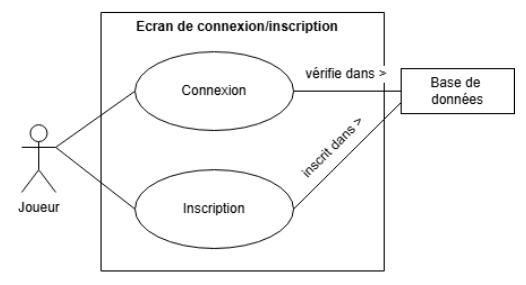
\includegraphics[width=0.4\textwidth, keepaspectratio]{src/design/connexion_design.png}
    \caption{Use-Case : Connexion}
    \label{fig:use_case_connexion_design}
\end{figure}

\section{Gestion des comptes}

\noindent Une fois qu’un joueur crée un compte, celui-ci est stocké dans la base de données. Cela permet à l'utilisateur d'accéder aux fonctionnalités du jeu, telles que le chat et la gestion de sa liste d'amis.

% diagramme gestion compte

\section{Gestion du profil}

\noindent Cette interface permet aux joueurs de modifier des informations personnelles, telles que leur mot de passe et leur pseudo. Les modifications apportées sont immédiatement enregistrées dans la base de données.

\vspace{-1em}

\begin{figure}[H]
    \centering
     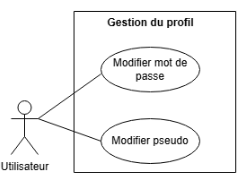
\includegraphics[width=0.4\textwidth, keepaspectratio]{src/design/user.png}
    \caption{Use-Case : Gestion du Profil}
    \label{fig:use_case_profil_managing_design}
\end{figure}

\section{Menu principal}

\noindent Le menu principal permet d'accéder à différentes sections du jeu, telles que le lobby pour créer ou rejoindre une partie, ainsi que le classement des meilleurs joueurs. Ce menu est l'interface de navigation principale dans le jeu.

\section{Matchmaking}

\noindent Le serveur gère une liste de parties actives et une liste de parties en état de \emph{matchmaking}, c’est-à-dire des parties en attente de joueurs pour être complétées. Lorsqu'un joueur souhaite rejoindre une partie, le serveur vérifie s'ils existent déjà des parties en \emph{matchmaking}. Si au moins une partie est disponible, le joueur peut choisir de la rejoindre. Sinon, le serveur crée une nouvelle partie avec ce joueur comme premier participant et marque la partie comme étant en \emph{matchmaking}.

\vspace{-1em}

\begin{figure}[H]
    \centering
     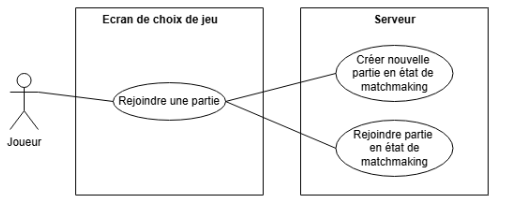
\includegraphics[width=0.6\textwidth, keepaspectratio]{src/design/matchmaking.png}
    \caption{Use-Case : Matchmaking}
    \label{fig:use_case_matchmaking}
\end{figure}

\section{Chat}

\noindent Le jeu propose un système de chat permettant aux joueurs d'envoyer des messages privés à ceux présents dans leur liste d'amis. Les messages envoyés passent par un contrôle pour bloquer les liens malicieux ou les insultes, assurant ainsi une expérience de communication respectueuese et adaptée à tous.

\section{Jeu}

\noindent Dans le mode de jeu, les joueurs débutent avec un plateau vide sur lequel des tétraminos tombent. Grâce aux commandes du jeu, ils doivent déplacer les tétraminos pour les positionner de manière stratégique. Les états des parties sont sauvegardés côté serveur, et les actions des joueurs sont envoyées au serveur pour validation. \\

\noindent Le joueur n'a jamais d'accès direct à sa partie. Toutes les interactions passent par le \emph{GameEngine}, qui gère la logique du jeu afin d'assurer la sécurité et d'empêcher la triche. Le serveur garde une vue d'ensemble des parties des joueurs dans la session en cours, ce qui lui permet de déterminer la fin d'une partie (par exemple, lorsque seulement un joueur reste en vie dans le mode Royal).

\noindent Même en mode solo, les joueurs doivent se connecter au serveur, ce qui permet de bénéficier de certaines fonctionnalités, comme l’observation des parties en cours.

\section{Vue globale}

\noindent Dans cette section, nous présenterons les diagrammes de classes et les diagrammes de cas d’utilisation (\textit{Use-Case}) associés à la vue globale du projet.

\subsection{Vue globale : MVC}

\vspace{-1em}

\begin{figure}[H]
    \centering
    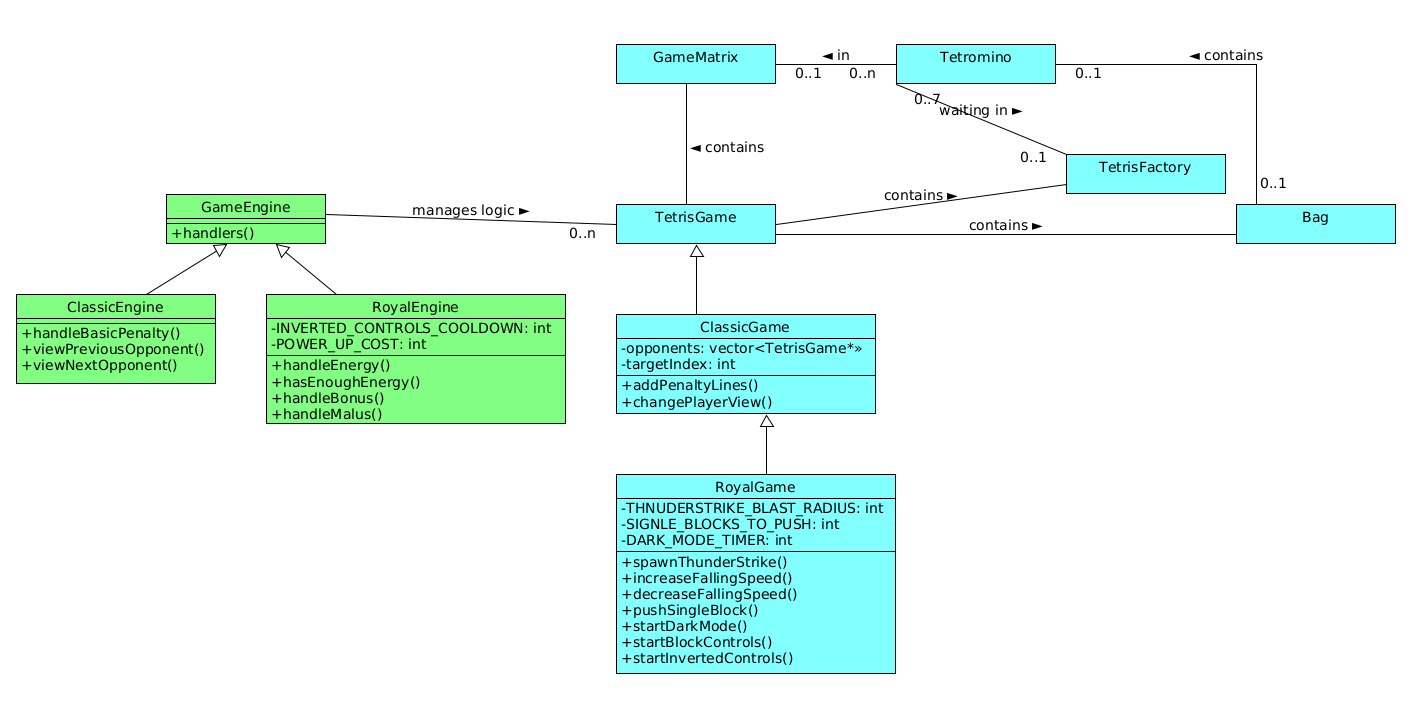
\includegraphics[width=\textwidth, keepaspectratio]{src/global.png}
    \caption{Diagramme de classes : Vue globale du système en architecture MVC}
    \label{fig:class_global_mvc}
\end{figure}

\subsubsection{Vue globale : Vue}

\subsection{Vue globale : Serveur}

\vspace{-1em}

\begin{figure}[H]
    \centering
    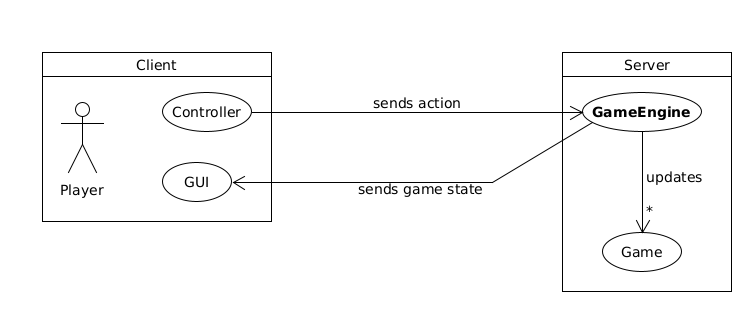
\includegraphics[width=\textwidth, keepaspectratio]{src/server.png}
    \caption{Diagramme de cas d’utilisation : Interactions client-serveur}
    \label{fig:use_case_server}
\end{figure}

\vspace{-1em}

\begin{figure}[H]
    \centering
    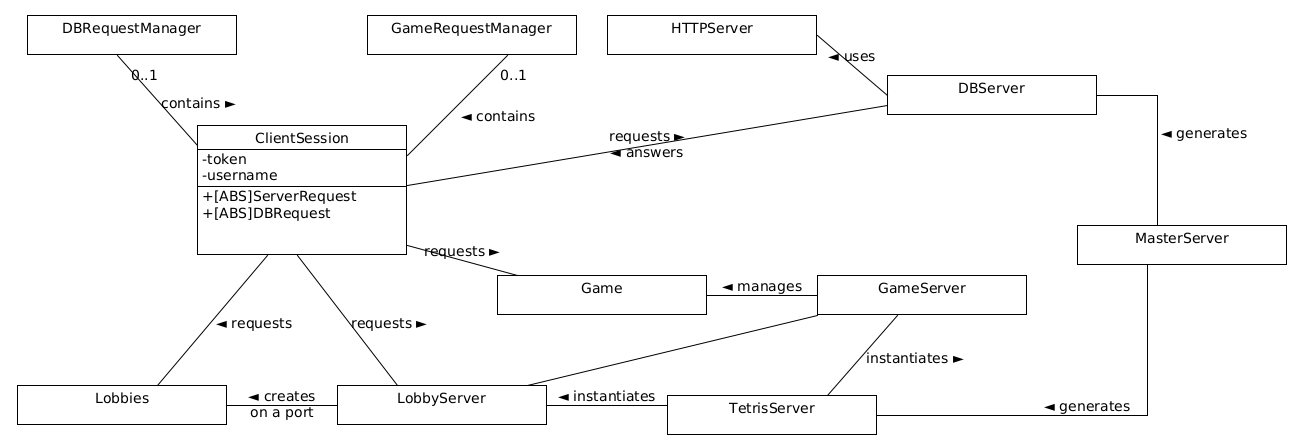
\includegraphics[width=\textwidth, keepaspectratio]{src/server_class.png}
    \caption{Diagramme de classes : Interactions classes du serveur}
    \label{fig:classes_server}
\end{figure}

\subsection{Vue globale : Base de données}

\vspace{-1em}

\begin{figure}[H]
    \centering
    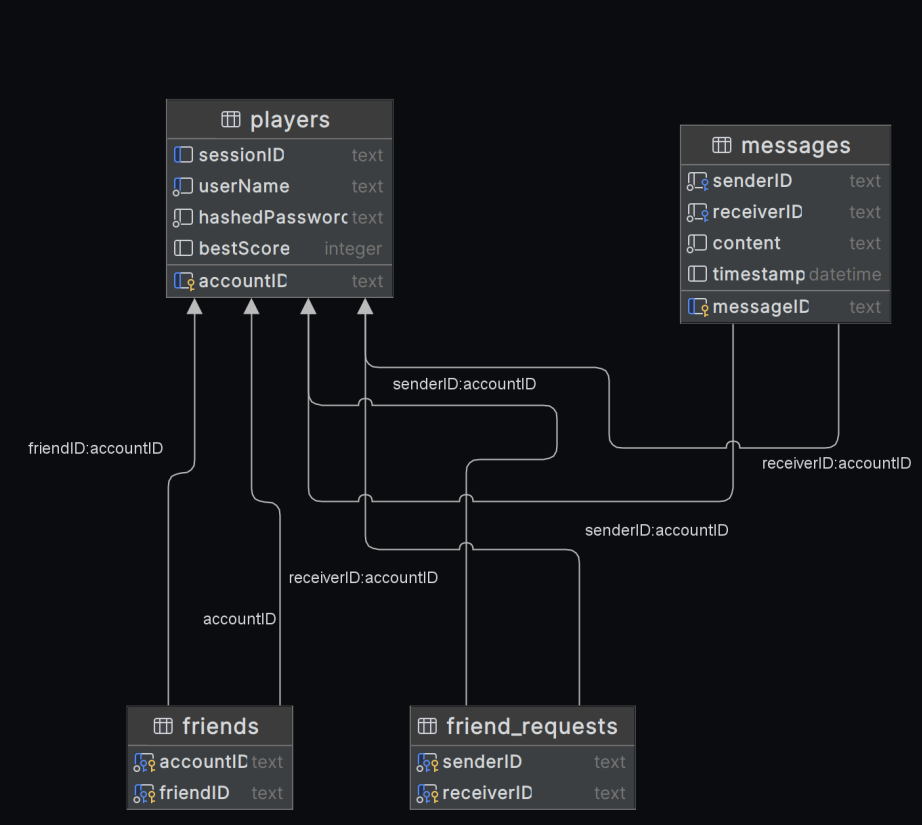
\includegraphics[width=\textwidth, keepaspectratio]{src/db.png}
    \caption{Diagramme entité-relation : Base de données}
    \label{fig:entity_relation_database}
\end{figure}
+

\end{document}